%% Font size %%
\documentclass[11pt]{article}

%% Load the custom package
\usepackage{Mathdoc}

%% Numéro de séquence %% Titre de la séquence %%
\renewcommand{\centerhead}{Extremum}

%% Spacing commands %%
\renewcommand{\baselinestretch}{1}
\setlength{\parindent}{0pt}

\begin{document}

\section{Recherche d'extremum}

\begin{exercice}[1][Formes cannoniques]
  \begin{enu}
\item On considère la fonction $f$ définie sur $\R$ par : $f(x)=5\left(x +\dfrac{9}{2}\right)^2 -\dfrac{441}{4}$.\\Déterminer l'extremum de la fonction $f$ ainsi que son image. 
	\item On considère la fonction $f$ définie sur $\R$ par : $f(x)=-3\left(x +5\right)^2 +68$.\\Déterminer l'extremum de la fonction $f$ ainsi que son image. 
	\item On considère la fonction $f$ définie sur $\R$ par : $f(x)=4\left(x +\dfrac{9}{2}\right)^2 -84$.\\Déterminer l'extremum de la fonction $f$ ainsi que son image. 
	\item On considère la fonction $f$ définie sur $\R$ par : $f(x)=-\left(x -5\right)^2 +22$.\\Déterminer l'extremum de la fonction $f$ ainsi que son image. 
  \end{enu}
\end{exercice}

\begin{exercice}[2][Formes développées]
  \begin{enu}
    \item On considère la fonction $f$ définie sur $\R$ par : $f(x)=5x^2+45x-9$.\\Déterminer l'extremum de la fonction $f$ ainsi que son image. 
	\item On considère la fonction $f$ définie sur $\R$ par : $f(x)=-3x^2-30x-7$.\\Déterminer l'extremum de la fonction $f$ ainsi que son image. 
	\item On considère la fonction $f$ définie sur $\R$ par : $f(x)=4x^2+36x-3$.\\Déterminer l'extremum de la fonction $f$ ainsi que son image. 
	\item On considère la fonction $f$ définie sur $\R$ par : $f(x)=-x^2+10x-3$.\\Déterminer l'extremum de la fonction $f$ ainsi que son image. 
  \end{enu}
\end{exercice}

\begin{exercice}[3][Formes factorisées]
  \begin{enu}
\item On considère la fonction $f$ définie sur $\R$ par : $f(x)=-3(x-5)(x-9)$.\\Déterminer l'extremum de la fonction $f$ ainsi que son image. 
	\item On considère la fonction $f$ définie sur $\R$ par : $f(x)=-2(x-1)(x-7)$.\\Déterminer l'extremum de la fonction $f$ ainsi que son image. 
	\item On considère la fonction $f$ définie sur $\R$ par : $f(x)=2(x-3)(x-5)$.\\Déterminer l'extremum de la fonction $f$ ainsi que son image. 
	\item On considère la fonction $f$ définie sur $\R$ par : $f(x)=3(x+1)(x-1)$.\\Déterminer l'extremum de la fonction $f$ ainsi que son image. 

  \end{enu}
\end{exercice}

\section{Lecture graphique}

\begin{exercice}[2][Répondre à ces questions par lecture graphique.]
  \begin{multicols}{2}
    \begin{enumerate}
    \item Quelles sont les coordonnées du sommet de la fonction
      polynomiale $\mathscr{f}$ du second degré représentée ci-dessous
      ?\\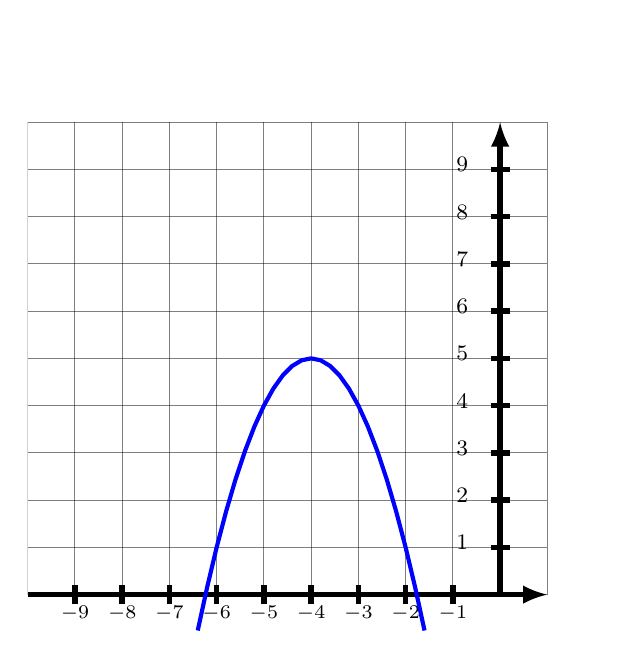
\begin{tikzpicture}[baseline,scale = 0.6]

        \tikzset{ point/.style={ thick, draw, cross out, inner
            sep=0pt, minimum width=5pt, minimum height=5pt, }, } \clip
        (-10,-1) rectangle (2,12);
    	
	\draw[color ={black},line width = 2,>=latex,->]
        (-10,0)--(1,0); \draw[color ={black},line width =
        2,>=latex,->] (0,0)--(0,10); \draw[color ={black},opacity =
        0.5] (-10,1)--(1,1); \draw[color ={black},opacity = 0.5]
        (-10,2)--(1,2); \draw[color ={black},opacity = 0.5]
        (-10,3)--(1,3); \draw[color ={black},opacity = 0.5]
        (-10,4)--(1,4); \draw[color ={black},opacity = 0.5]
        (-10,5)--(1,5); \draw[color ={black},opacity = 0.5]
        (-10,6)--(1,6); \draw[color ={black},opacity = 0.5]
        (-10,7)--(1,7); \draw[color ={black},opacity = 0.5]
        (-10,8)--(1,8); \draw[color ={black},opacity = 0.5]
        (-10,9)--(1,9); \draw[color ={black},opacity = 0.5]
        (-10,10)--(1,10); \draw[color ={black},opacity = 0.5]
        (1,0)--(1,10); \draw[color ={black},opacity = 0.5]
        (-1,0)--(-1,10); \draw[color ={black},opacity = 0.5]
        (-2,0)--(-2,10); \draw[color ={black},opacity = 0.5]
        (-3,0)--(-3,10); \draw[color ={black},opacity = 0.5]
        (-4,0)--(-4,10); \draw[color ={black},opacity = 0.5]
        (-5,0)--(-5,10); \draw[color ={black},opacity = 0.5]
        (-6,0)--(-6,10); \draw[color ={black},opacity = 0.5]
        (-7,0)--(-7,10); \draw[color ={black},opacity = 0.5]
        (-8,0)--(-8,10); \draw[color ={black},opacity = 0.5]
        (-9,0)--(-9,10); \draw[color ={black},opacity = 0.5]
        (-10,0)--(-10,10); \draw[color ={black},line width = 2]
        (-1,-0.2)--(-1,0.2); \draw[color ={black},line width = 2]
        (-2,-0.2)--(-2,0.2); \draw[color ={black},line width = 2]
        (-3,-0.2)--(-3,0.2); \draw[color ={black},line width = 2]
        (-4,-0.2)--(-4,0.2); \draw[color ={black},line width = 2]
        (-5,-0.2)--(-5,0.2); \draw[color ={black},line width = 2]
        (-6,-0.2)--(-6,0.2); \draw[color ={black},line width = 2]
        (-7,-0.2)--(-7,0.2); \draw[color ={black},line width = 2]
        (-8,-0.2)--(-8,0.2); \draw[color ={black},line width = 2]
        (-9,-0.2)--(-9,0.2); \draw[color ={black},line width = 2]
        (-0.2,1)--(0.2,1); \draw[color ={black},line width = 2]
        (-0.2,2)--(0.2,2); \draw[color ={black},line width = 2]
        (-0.2,3)--(0.2,3); \draw[color ={black},line width = 2]
        (-0.2,4)--(0.2,4); \draw[color ={black},line width = 2]
        (-0.2,5)--(0.2,5); \draw[color ={black},line width = 2]
        (-0.2,6)--(0.2,6); \draw[color ={black},line width = 2]
        (-0.2,7)--(0.2,7); \draw[color ={black},line width = 2]
        (-0.2,8)--(0.2,8); \draw[color ={black},line width = 2]
        (-0.2,9)--(0.2,9); \draw (-1,-0.4) node[anchor = center]
        {\scriptsize \color{black}{$-1$}}; \draw (-2,-0.4) node[anchor
        = center] {\scriptsize \color{black}{$-2$}}; \draw (-3,-0.4)
        node[anchor = center] {\scriptsize \color{black}{$-3$}}; \draw
        (-4,-0.4) node[anchor = center] {\scriptsize
          \color{black}{$-4$}}; \draw (-5,-0.4) node[anchor = center]
        {\scriptsize \color{black}{$-5$}}; \draw (-6,-0.4) node[anchor
        = center] {\scriptsize \color{black}{$-6$}}; \draw (-7,-0.4)
        node[anchor = center] {\scriptsize \color{black}{$-7$}}; \draw
        (-8,-0.4) node[anchor = center] {\scriptsize
          \color{black}{$-8$}}; \draw (-9,-0.4) node[anchor = center]
        {\scriptsize \color{black}{$-9$}}; \draw (-0.8,1.1)
        node[anchor = center] {\footnotesize \color{black}{$1$}};
        \draw (-0.8,2.1) node[anchor = center] {\footnotesize
          \color{black}{$2$}}; \draw (-0.8,3.1) node[anchor = center]
        {\footnotesize \color{black}{$3$}}; \draw (-0.8,4.1)
        node[anchor = center] {\footnotesize \color{black}{$4$}};
        \draw (-0.8,5.1) node[anchor = center] {\footnotesize
          \color{black}{$5$}}; \draw (-0.8,6.1) node[anchor = center]
        {\footnotesize \color{black}{$6$}}; \draw (-0.8,7.1)
        node[anchor = center] {\footnotesize \color{black}{$7$}};
        \draw (-0.8,8.1) node[anchor = center] {\footnotesize
          \color{black}{$8$}}; \draw (-0.8,9.1) node[anchor = center]
        {\footnotesize \color{black}{$9$}};
	
	\draw[color={blue},line width = 1.5]
        (-6.4,-0.76)--(-6.2,0.16)--(-6,1)--(-5.8,1.76)--(-5.6,2.44)--(-5.4,3.04)--(-5.2,3.56)--(-5,4)--(-4.8,4.36)--(-4.6,4.64)--(-4.4,4.84)--(-4.2,4.96)--(-4,5)--(-3.8,4.96)--(-3.6,4.84)--(-3.4,4.64)--(-3.2,4.36)--(-3,4)--(-2.8,3.56)--(-2.6,3.04)--(-2.4,2.44)--(-2.2,1.76)--(-2,1)--(-1.8,0.16)--(-1.6,-0.76);

      \end{tikzpicture}\\
    \item Quelles sont les coordonnées du sommet de la fonction
      polynomiale $\mathscr{g}$ du second degré représentée ci-dessous
      ?\\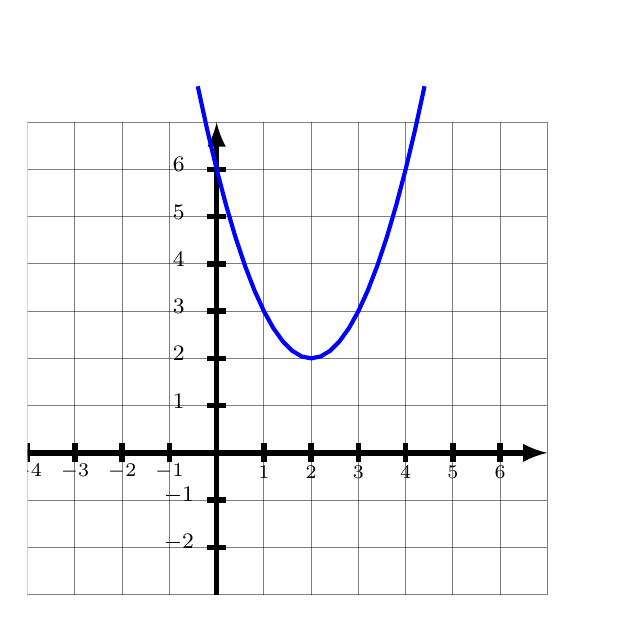
\begin{tikzpicture}[baseline,scale = 0.6]

        \tikzset{ point/.style={ thick, draw, cross out, inner
            sep=0pt, minimum width=5pt, minimum height=5pt, }, } \clip
        (-4,-3) rectangle (8,9);
    	
	\draw[color ={black},line width = 2,>=latex,->]
        (-10,0)--(7,0); \draw[color ={black},line width =
        2,>=latex,->] (0,-3)--(0,7); \draw[color ={black},opacity =
        0.5] (-10,1)--(7,1); \draw[color ={black},opacity = 0.5]
        (-10,2)--(7,2); \draw[color ={black},opacity = 0.5]
        (-10,3)--(7,3); \draw[color ={black},opacity = 0.5]
        (-10,4)--(7,4); \draw[color ={black},opacity = 0.5]
        (-10,5)--(7,5); \draw[color ={black},opacity = 0.5]
        (-10,6)--(7,6); \draw[color ={black},opacity = 0.5]
        (-10,7)--(7,7); \draw[color ={black},opacity = 0.5]
        (-10,-1)--(7,-1); \draw[color ={black},opacity = 0.5]
        (-10,-2)--(7,-2); \draw[color ={black},opacity = 0.5]
        (-10,-3)--(7,-3); \draw[color ={black},opacity = 0.5]
        (1,-3)--(1,7); \draw[color ={black},opacity = 0.5]
        (2,-3)--(2,7); \draw[color ={black},opacity = 0.5]
        (3,-3)--(3,7); \draw[color ={black},opacity = 0.5]
        (4,-3)--(4,7); \draw[color ={black},opacity = 0.5]
        (5,-3)--(5,7); \draw[color ={black},opacity = 0.5]
        (6,-3)--(6,7); \draw[color ={black},opacity = 0.5]
        (7,-3)--(7,7); \draw[color ={black},opacity = 0.5]
        (-1,-3)--(-1,7); \draw[color ={black},opacity = 0.5]
        (-2,-3)--(-2,7); \draw[color ={black},opacity = 0.5]
        (-3,-3)--(-3,7); \draw[color ={black},opacity = 0.5]
        (-4,-3)--(-4,7); \draw[color ={black},opacity = 0.5]
        (-5,-3)--(-5,7); \draw[color ={black},opacity = 0.5]
        (-6,-3)--(-6,7); \draw[color ={black},opacity = 0.5]
        (-7,-3)--(-7,7); \draw[color ={black},opacity = 0.5]
        (-8,-3)--(-8,7); \draw[color ={black},opacity = 0.5]
        (-9,-3)--(-9,7); \draw[color ={black},opacity = 0.5]
        (-10,-3)--(-10,7); \draw[color ={black},line width = 2]
        (1,-0.2)--(1,0.2); \draw[color ={black},line width = 2]
        (2,-0.2)--(2,0.2); \draw[color ={black},line width = 2]
        (3,-0.2)--(3,0.2); \draw[color ={black},line width = 2]
        (4,-0.2)--(4,0.2); \draw[color ={black},line width = 2]
        (5,-0.2)--(5,0.2); \draw[color ={black},line width = 2]
        (6,-0.2)--(6,0.2); \draw[color ={black},line width = 2]
        (-1,-0.2)--(-1,0.2); \draw[color ={black},line width = 2]
        (-2,-0.2)--(-2,0.2); \draw[color ={black},line width = 2]
        (-3,-0.2)--(-3,0.2); \draw[color ={black},line width = 2]
        (-4,-0.2)--(-4,0.2); \draw[color ={black},line width = 2]
        (-5,-0.2)--(-5,0.2); \draw[color ={black},line width = 2]
        (-6,-0.2)--(-6,0.2); \draw[color ={black},line width = 2]
        (-7,-0.2)--(-7,0.2); \draw[color ={black},line width = 2]
        (-8,-0.2)--(-8,0.2); \draw[color ={black},line width = 2]
        (-9,-0.2)--(-9,0.2); \draw[color ={black},line width = 2]
        (-0.2,1)--(0.2,1); \draw[color ={black},line width = 2]
        (-0.2,2)--(0.2,2); \draw[color ={black},line width = 2]
        (-0.2,3)--(0.2,3); \draw[color ={black},line width = 2]
        (-0.2,4)--(0.2,4); \draw[color ={black},line width = 2]
        (-0.2,5)--(0.2,5); \draw[color ={black},line width = 2]
        (-0.2,6)--(0.2,6); \draw[color ={black},line width = 2]
        (-0.2,-1)--(0.2,-1); \draw[color ={black},line width = 2]
        (-0.2,-2)--(0.2,-2); \draw (1,-0.4) node[anchor = center]
        {\scriptsize \color{black}{$1$}}; \draw (2,-0.4) node[anchor =
        center] {\scriptsize \color{black}{$2$}}; \draw (3,-0.4)
        node[anchor = center] {\scriptsize \color{black}{$3$}}; \draw
        (4,-0.4) node[anchor = center] {\scriptsize
          \color{black}{$4$}}; \draw (5,-0.4) node[anchor = center]
        {\scriptsize \color{black}{$5$}}; \draw (6,-0.4) node[anchor =
        center] {\scriptsize \color{black}{$6$}}; \draw (-1,-0.4)
        node[anchor = center] {\scriptsize \color{black}{$-1$}}; \draw
        (-2,-0.4) node[anchor = center] {\scriptsize
          \color{black}{$-2$}}; \draw (-3,-0.4) node[anchor = center]
        {\scriptsize \color{black}{$-3$}}; \draw (-4,-0.4) node[anchor
        = center] {\scriptsize \color{black}{$-4$}}; \draw (-5,-0.4)
        node[anchor = center] {\scriptsize \color{black}{$-5$}}; \draw
        (-6,-0.4) node[anchor = center] {\scriptsize
          \color{black}{$-6$}}; \draw (-7,-0.4) node[anchor = center]
        {\scriptsize \color{black}{$-7$}}; \draw (-8,-0.4) node[anchor
        = center] {\scriptsize \color{black}{$-8$}}; \draw (-9,-0.4)
        node[anchor = center] {\scriptsize \color{black}{$-9$}}; \draw
        (-0.8,1.1) node[anchor = center] {\footnotesize
          \color{black}{$1$}}; \draw (-0.8,2.1) node[anchor = center]
        {\footnotesize \color{black}{$2$}}; \draw (-0.8,3.1)
        node[anchor = center] {\footnotesize \color{black}{$3$}};
        \draw (-0.8,4.1) node[anchor = center] {\footnotesize
          \color{black}{$4$}}; \draw (-0.8,5.1) node[anchor = center]
        {\footnotesize \color{black}{$5$}}; \draw (-0.8,6.1)
        node[anchor = center] {\footnotesize \color{black}{$6$}};
        \draw (-0.8,-0.9) node[anchor = center] {\footnotesize
          \color{black}{$-1$}}; \draw (-0.8,-1.9) node[anchor =
        center] {\footnotesize \color{black}{$-2$}};
	
	\draw[color={blue},line width = 1.5]
        (-0.4,7.76)--(-0.2,6.84)--(0,6)--(0.2,5.24)--(0.4,4.56)--(0.6,3.96)--(0.8,3.44)--(1,3)--(1.2,2.64)--(1.4,2.36)--(1.6,2.16)--(1.8,2.04)--(2,2)--(2.2,2.04)--(2.4,2.16)--(2.6,2.36)--(2.8,2.64)--(3,3)--(3.2,3.44)--(3.4,3.96)--(3.6,4.56)--(3.8,5.24)--(4,6)--(4.2,6.84)--(4.4,7.76);

      \end{tikzpicture}\\
    \item Quelles sont les coordonnées du sommet de la fonction
      polynomiale $\mathscr{i}$ du second degré représentée ci-dessous
      ?\\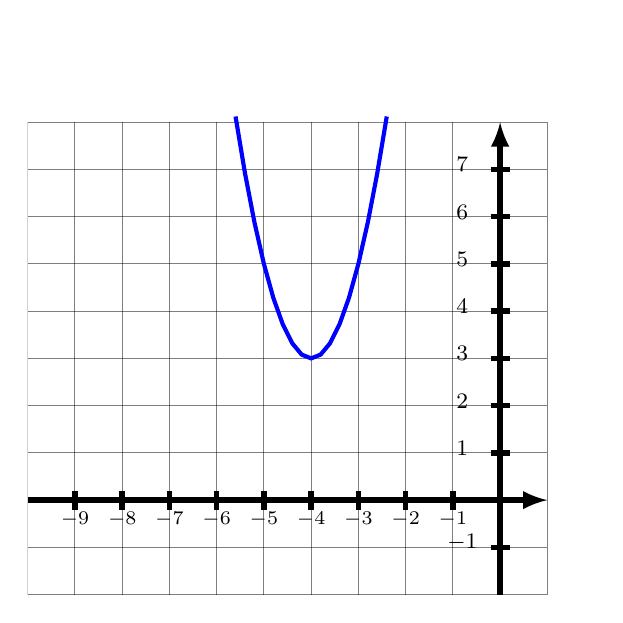
\begin{tikzpicture}[baseline,scale = 0.6]

        \tikzset{ point/.style={ thick, draw, cross out, inner
            sep=0pt, minimum width=5pt, minimum height=5pt, }, } \clip
        (-10,-2) rectangle (2,10);
    	
	\draw[color ={black},line width = 2,>=latex,->]
        (-10,0)--(1,0); \draw[color ={black},line width =
        2,>=latex,->] (0,-2)--(0,8); \draw[color ={black},opacity =
        0.5] (-10,1)--(1,1); \draw[color ={black},opacity = 0.5]
        (-10,2)--(1,2); \draw[color ={black},opacity = 0.5]
        (-10,3)--(1,3); \draw[color ={black},opacity = 0.5]
        (-10,4)--(1,4); \draw[color ={black},opacity = 0.5]
        (-10,5)--(1,5); \draw[color ={black},opacity = 0.5]
        (-10,6)--(1,6); \draw[color ={black},opacity = 0.5]
        (-10,7)--(1,7); \draw[color ={black},opacity = 0.5]
        (-10,8)--(1,8); \draw[color ={black},opacity = 0.5]
        (-10,-1)--(1,-1); \draw[color ={black},opacity = 0.5]
        (-10,-2)--(1,-2); \draw[color ={black},opacity = 0.5]
        (1,-2)--(1,8); \draw[color ={black},opacity = 0.5]
        (-1,-2)--(-1,8); \draw[color ={black},opacity = 0.5]
        (-2,-2)--(-2,8); \draw[color ={black},opacity = 0.5]
        (-3,-2)--(-3,8); \draw[color ={black},opacity = 0.5]
        (-4,-2)--(-4,8); \draw[color ={black},opacity = 0.5]
        (-5,-2)--(-5,8); \draw[color ={black},opacity = 0.5]
        (-6,-2)--(-6,8); \draw[color ={black},opacity = 0.5]
        (-7,-2)--(-7,8); \draw[color ={black},opacity = 0.5]
        (-8,-2)--(-8,8); \draw[color ={black},opacity = 0.5]
        (-9,-2)--(-9,8); \draw[color ={black},opacity = 0.5]
        (-10,-2)--(-10,8); \draw[color ={black},line width = 2]
        (-1,-0.2)--(-1,0.2); \draw[color ={black},line width = 2]
        (-2,-0.2)--(-2,0.2); \draw[color ={black},line width = 2]
        (-3,-0.2)--(-3,0.2); \draw[color ={black},line width = 2]
        (-4,-0.2)--(-4,0.2); \draw[color ={black},line width = 2]
        (-5,-0.2)--(-5,0.2); \draw[color ={black},line width = 2]
        (-6,-0.2)--(-6,0.2); \draw[color ={black},line width = 2]
        (-7,-0.2)--(-7,0.2); \draw[color ={black},line width = 2]
        (-8,-0.2)--(-8,0.2); \draw[color ={black},line width = 2]
        (-9,-0.2)--(-9,0.2); \draw[color ={black},line width = 2]
        (-0.2,1)--(0.2,1); \draw[color ={black},line width = 2]
        (-0.2,2)--(0.2,2); \draw[color ={black},line width = 2]
        (-0.2,3)--(0.2,3); \draw[color ={black},line width = 2]
        (-0.2,4)--(0.2,4); \draw[color ={black},line width = 2]
        (-0.2,5)--(0.2,5); \draw[color ={black},line width = 2]
        (-0.2,6)--(0.2,6); \draw[color ={black},line width = 2]
        (-0.2,7)--(0.2,7); \draw[color ={black},line width = 2]
        (-0.2,-1)--(0.2,-1); \draw (-1,-0.4) node[anchor = center]
        {\scriptsize \color{black}{$-1$}}; \draw (-2,-0.4) node[anchor
        = center] {\scriptsize \color{black}{$-2$}}; \draw (-3,-0.4)
        node[anchor = center] {\scriptsize \color{black}{$-3$}}; \draw
        (-4,-0.4) node[anchor = center] {\scriptsize
          \color{black}{$-4$}}; \draw (-5,-0.4) node[anchor = center]
        {\scriptsize \color{black}{$-5$}}; \draw (-6,-0.4) node[anchor
        = center] {\scriptsize \color{black}{$-6$}}; \draw (-7,-0.4)
        node[anchor = center] {\scriptsize \color{black}{$-7$}}; \draw
        (-8,-0.4) node[anchor = center] {\scriptsize
          \color{black}{$-8$}}; \draw (-9,-0.4) node[anchor = center]
        {\scriptsize \color{black}{$-9$}}; \draw (-0.8,1.1)
        node[anchor = center] {\footnotesize \color{black}{$1$}};
        \draw (-0.8,2.1) node[anchor = center] {\footnotesize
          \color{black}{$2$}}; \draw (-0.8,3.1) node[anchor = center]
        {\footnotesize \color{black}{$3$}}; \draw (-0.8,4.1)
        node[anchor = center] {\footnotesize \color{black}{$4$}};
        \draw (-0.8,5.1) node[anchor = center] {\footnotesize
          \color{black}{$5$}}; \draw (-0.8,6.1) node[anchor = center]
        {\footnotesize \color{black}{$6$}}; \draw (-0.8,7.1)
        node[anchor = center] {\footnotesize \color{black}{$7$}};
        \draw (-0.8,-0.9) node[anchor = center] {\footnotesize
          \color{black}{$-1$}};
	
	\draw[color={blue},line width = 1.5]
        (-5.6,8.12)--(-5.4,6.92)--(-5.2,5.88)--(-5,5)--(-4.8,4.28)--(-4.6,3.72)--(-4.4,3.32)--(-4.2,3.08)--(-4,3)--(-3.8,3.08)--(-3.6,3.32)--(-3.4,3.72)--(-3.2,4.28)--(-3,5)--(-2.8,5.88)--(-2.6,6.92)--(-2.4,8.12);

      \end{tikzpicture}\\
    \item Quelles sont les coordonnées du sommet de la fonction
      polynomiale $\mathscr{j}$ du second degré représentée ci-dessous
      ?\\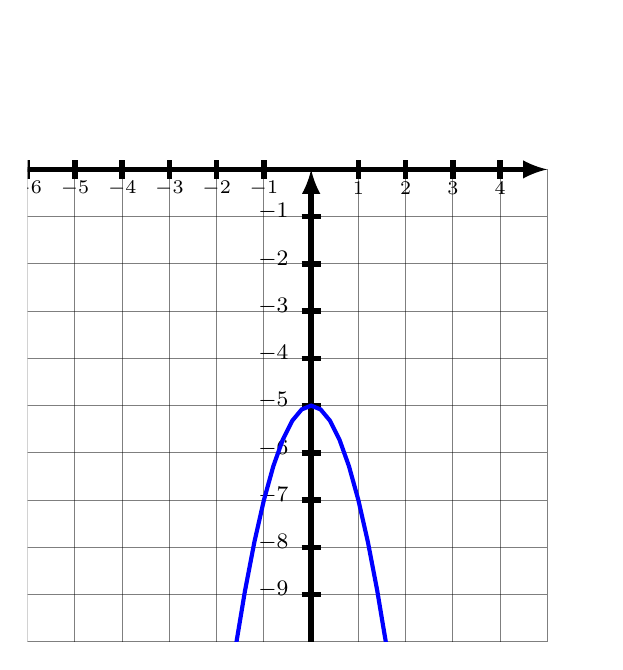
\begin{tikzpicture}[baseline,scale = 0.6]

        \tikzset{ point/.style={ thick, draw, cross out, inner
            sep=0pt, minimum width=5pt, minimum height=5pt, }, } \clip
        (-6,-10) rectangle (6,3);
    	
	\draw[color ={black},line width = 2,>=latex,->]
        (-10,0)--(5,0); \draw[color ={black},line width =
        2,>=latex,->] (0,-10)--(0,0); \draw[color ={black},opacity =
        0.5] (-10,-1)--(5,-1); \draw[color ={black},opacity = 0.5]
        (-10,-2)--(5,-2); \draw[color ={black},opacity = 0.5]
        (-10,-3)--(5,-3); \draw[color ={black},opacity = 0.5]
        (-10,-4)--(5,-4); \draw[color ={black},opacity = 0.5]
        (-10,-5)--(5,-5); \draw[color ={black},opacity = 0.5]
        (-10,-6)--(5,-6); \draw[color ={black},opacity = 0.5]
        (-10,-7)--(5,-7); \draw[color ={black},opacity = 0.5]
        (-10,-8)--(5,-8); \draw[color ={black},opacity = 0.5]
        (-10,-9)--(5,-9); \draw[color ={black},opacity = 0.5]
        (-10,-10)--(5,-10); \draw[color ={black},opacity = 0.5]
        (1,-10)--(1,0); \draw[color ={black},opacity = 0.5]
        (2,-10)--(2,0); \draw[color ={black},opacity = 0.5]
        (3,-10)--(3,0); \draw[color ={black},opacity = 0.5]
        (4,-10)--(4,0); \draw[color ={black},opacity = 0.5]
        (5,-10)--(5,0); \draw[color ={black},opacity = 0.5]
        (-1,-10)--(-1,0); \draw[color ={black},opacity = 0.5]
        (-2,-10)--(-2,0); \draw[color ={black},opacity = 0.5]
        (-3,-10)--(-3,0); \draw[color ={black},opacity = 0.5]
        (-4,-10)--(-4,0); \draw[color ={black},opacity = 0.5]
        (-5,-10)--(-5,0); \draw[color ={black},opacity = 0.5]
        (-6,-10)--(-6,0); \draw[color ={black},opacity = 0.5]
        (-7,-10)--(-7,0); \draw[color ={black},opacity = 0.5]
        (-8,-10)--(-8,0); \draw[color ={black},opacity = 0.5]
        (-9,-10)--(-9,0); \draw[color ={black},opacity = 0.5]
        (-10,-10)--(-10,0); \draw[color ={black},line width = 2]
        (1,-0.2)--(1,0.2); \draw[color ={black},line width = 2]
        (2,-0.2)--(2,0.2); \draw[color ={black},line width = 2]
        (3,-0.2)--(3,0.2); \draw[color ={black},line width = 2]
        (4,-0.2)--(4,0.2); \draw[color ={black},line width = 2]
        (-1,-0.2)--(-1,0.2); \draw[color ={black},line width = 2]
        (-2,-0.2)--(-2,0.2); \draw[color ={black},line width = 2]
        (-3,-0.2)--(-3,0.2); \draw[color ={black},line width = 2]
        (-4,-0.2)--(-4,0.2); \draw[color ={black},line width = 2]
        (-5,-0.2)--(-5,0.2); \draw[color ={black},line width = 2]
        (-6,-0.2)--(-6,0.2); \draw[color ={black},line width = 2]
        (-7,-0.2)--(-7,0.2); \draw[color ={black},line width = 2]
        (-8,-0.2)--(-8,0.2); \draw[color ={black},line width = 2]
        (-9,-0.2)--(-9,0.2); \draw[color ={black},line width = 2]
        (-0.2,-1)--(0.2,-1); \draw[color ={black},line width = 2]
        (-0.2,-2)--(0.2,-2); \draw[color ={black},line width = 2]
        (-0.2,-3)--(0.2,-3); \draw[color ={black},line width = 2]
        (-0.2,-4)--(0.2,-4); \draw[color ={black},line width = 2]
        (-0.2,-5)--(0.2,-5); \draw[color ={black},line width = 2]
        (-0.2,-6)--(0.2,-6); \draw[color ={black},line width = 2]
        (-0.2,-7)--(0.2,-7); \draw[color ={black},line width = 2]
        (-0.2,-8)--(0.2,-8); \draw[color ={black},line width = 2]
        (-0.2,-9)--(0.2,-9); \draw (1,-0.4) node[anchor = center]
        {\scriptsize \color{black}{$1$}}; \draw (2,-0.4) node[anchor =
        center] {\scriptsize \color{black}{$2$}}; \draw (3,-0.4)
        node[anchor = center] {\scriptsize \color{black}{$3$}}; \draw
        (4,-0.4) node[anchor = center] {\scriptsize
          \color{black}{$4$}}; \draw (-1,-0.4) node[anchor = center]
        {\scriptsize \color{black}{$-1$}}; \draw (-2,-0.4) node[anchor
        = center] {\scriptsize \color{black}{$-2$}}; \draw (-3,-0.4)
        node[anchor = center] {\scriptsize \color{black}{$-3$}}; \draw
        (-4,-0.4) node[anchor = center] {\scriptsize
          \color{black}{$-4$}}; \draw (-5,-0.4) node[anchor = center]
        {\scriptsize \color{black}{$-5$}}; \draw (-6,-0.4) node[anchor
        = center] {\scriptsize \color{black}{$-6$}}; \draw (-7,-0.4)
        node[anchor = center] {\scriptsize \color{black}{$-7$}}; \draw
        (-8,-0.4) node[anchor = center] {\scriptsize
          \color{black}{$-8$}}; \draw (-9,-0.4) node[anchor = center]
        {\scriptsize \color{black}{$-9$}}; \draw (-0.8,-0.9)
        node[anchor = center] {\footnotesize \color{black}{$-1$}};
        \draw (-0.8,-1.9) node[anchor = center] {\footnotesize
          \color{black}{$-2$}}; \draw (-0.8,-2.9) node[anchor =
        center] {\footnotesize \color{black}{$-3$}}; \draw (-0.8,-3.9)
        node[anchor = center] {\footnotesize \color{black}{$-4$}};
        \draw (-0.8,-4.9) node[anchor = center] {\footnotesize
          \color{black}{$-5$}}; \draw (-0.8,-5.9) node[anchor =
        center] {\footnotesize \color{black}{$-6$}}; \draw (-0.8,-6.9)
        node[anchor = center] {\footnotesize \color{black}{$-7$}};
        \draw (-0.8,-7.9) node[anchor = center] {\footnotesize
          \color{black}{$-8$}}; \draw (-0.8,-8.9) node[anchor =
        center] {\footnotesize \color{black}{$-9$}};
	
	\draw[color={blue},line width = 1.5]
        (-1.6,-10.12)--(-1.4,-8.92)--(-1.2,-7.88)--(-1,-7)--(-0.8,-6.28)--(-0.6,-5.72)--(-0.4,-5.32)--(-0.2,-5.08)--(0,-5)--(0.2,-5.08)--(0.4,-5.32)--(0.6,-5.72)--(0.8,-6.28)--(1,-7)--(1.2,-7.88)--(1.4,-8.92)--(1.6,-10.12);

      \end{tikzpicture}
 \end{enumerate}
\end{multicols}
\end{exercice}


\section{Tableaux de variations}

\begin{exercice}[0][Exercice Corrigé.]
 On considère la fonction $f$ définie sur $\R$ par :
 $f(x)=4x^2-20x-6$.\\
 Dresser le tableau de  variations de la fonction $f$ sur
 $\R$. \\
 \textbf{Correction.}
 \begin{enumerate}[label=(\arabic*)]
 \item On reconnaît la forme développée d'une fonction polynôme du
   second degré $ax^2+bx+c$ avec $a=4$, $b=-20$ et $c=-6$.
 \item Comme $a > 0$, la fonction est d'abord décroissante puis croissante.
 \item Le changement de variation s'opère en
   $\alpha=-\dfrac{b}{2a}=\dfrac{-(-20)}{2\times
     4}=\dfrac{5}{2}$. 
 \item De plus, $f\left(\dfrac{5}{2}\right)=4 \times \left(\dfrac{5}{2}
   \right)^2 -20 \times \dfrac{5}{2} -6 = -31$.
 \item On en déduit le tableau de variations de $f$ sur $\R$ :
   \begin{center}
     \begin{tikzpicture}[baseline, scale=0.75]
       \tkzTabInit[lgt=3,deltacl=0.8,espcl=4.5]{ $x$ / 1.5, $f(x)$ /
         3}{ $-\infty$, $\dfrac{5}{2}$, $+\infty$} \tkzTabVar{ +/ ,
         -/$-31$, +/ }
     \end{tikzpicture}
   \end{center}
 \end{enumerate}
\end{exercice}

\begin{exercice}[2][Tableaux de variations sur $\R$]
  \begin{enu}
    \item On considère la fonction $f$ définie sur $\R$ par : $f(x)=-x^2-7x+4$.\\Dresser le tableau de  variations de la fonction $f$ sur $\R$.
	\item On considère la fonction $f$ définie sur $\R$ par : $f(x)=3x(x+2)$.\\Dresser le tableau de  variations de la fonction $f$ sur $\R$.
	\item On considère la fonction $f$ définie sur $\R$ par : $f(x)=5\left(x -\dfrac{3}{2}\right)^2 -\dfrac{41}{4}$.\\Dresser le tableau de  variations de la fonction $f$ sur $\R$.
	\item On considère la fonction $f$ définie sur $\R$ par : $f(x)=-5\left(x -5\right)^2 +119$.\\Dresser le tableau de  variations de la fonction $f$ sur $\R$.
	\item On considère la fonction $f$ définie sur $\R$ par : $f(x)=3(x+1)(x-5)$.\\Dresser le tableau de  variations de la fonction $f$ sur $\R$.
  \end{enu}
\end{exercice}

\newpage

\phantom{0}
\vspace{-1cm}

\begin{exercice}[2][Tableaux de variations sur un intervalle borné]
  \begin{enu}
	\item On considère la fonction $f$ définie sur $[3\,;\,10]$ par : $f(x)=-x^2-7x+4$.\\Dresser le tableau de  variations de la fonction $f$ sur $[3\,;\,10]$.
	\item On considère la fonction $f$ définie sur $[1\,;\,6]$ par : $f(x)=3x(x+2)$.\\Dresser le tableau de  variations de la fonction $f$ sur $[1\,;\,6]$.
	\item On considère la fonction $f$ définie sur $[5\,;\,10]$ par : $f(x)=5\left(x -\dfrac{3}{2}\right)^2 -\dfrac{41}{4}$.\\Dresser le tableau de  variations de la fonction $f$ sur $[5\,;\,10]$.
	\item On considère la fonction $f$ définie sur $[0\,;\,7]$ par : $f(x)=-5\left(x -5\right)^2 +119$.\\Dresser le tableau de  variations de la fonction $f$ sur $[0\,;\,7]$.
	\item On considère la fonction $f$ définie sur $[4\,;\,6]$ par : $f(x)=3(x+1)(x-5)$.\\Dresser le tableau de  variations de la fonction $f$ sur $[4\,;\,6]$.
  \end{enu}
\end{exercice}

\vspace{-.5cm}

\begin{exercice}[3][Étude d'une fonction polynomiale]
  Soit $f(x)=\left(x +3\right)^2 -19$ un polynôme du second degré définie sur $\R$.
  \begin{enumerate}
  \item Déterminer le sens de variation de $f$ sur $\R$.
  \item Déterminer l'extremum de la fonction $f$ puis calculer son
    image.
  \item Dresser le tableau de variation de la fonction $f$ sur $\R$.
  \item Dans un repère orthonormé direct, représenter la fonction $f$ sur l'intervalle
    $[-7\,;\,1]$
  \end{enumerate}
\end{exercice}

\vspace{-.5cm}

\begin{exercice}[3][Étude d'une fonction polynomiale]
  Soit $f(x)=2x^2-2x-10$ un polynôme du second degré définie sur $\R$.
  \begin{enumerate}
  \item Déterminer le sens de variation de $f$ sur $\R$.
  \item Déterminer l'extremum de la fonction $f$ puis calculer son
    image.
  \item Dresser le tableau de variation de la fonction $f$ sur $\R$.
  \item Dans un repère orthonormé direct, représenter la fonction $f$ sur l'intervalle
    $[-4\,;\,4]$
  \end{enumerate}
\end{exercice}

\nopagebreak

\begin{exercice}[4][Étude d'une fonction polynomiale]
  Soit $f(x)=-2(x+1)(x-1)$ un polynôme du second degré définie sur $\R$.
  \begin{enumerate}
  \item Déterminer le sens de variation de $f$ sur $\R$.
  \item Déterminer l'extremum de la fonction $f$ puis calculer son
    image.
  \item Dresser le tableau de variation de la fonction $f$ sur $\R$.
  \item Dans un repère orthonormé direct, représenter la fonction $f$ sur l'intervalle
    $[-4\,;\,4]$
  \end{enumerate}
\end{exercice}


\end{document}

%%% Local Variables:
%%% mode: LaTeX
%%% TeX-master: t
%%% End:
